% template created by: Russell Haering. arr. Joseph Crop
\documentclass[12pt]{article}
\usepackage[hmargin=1in, vmargin=1in]{geometry}
\usepackage{fancyhdr}
\pagestyle{fancy}
\usepackage[hang,small]{caption}
\usepackage{lastpage}
\usepackage{graphicx}
\usepackage{verbatim}
\DeclareGraphicsExtensions{.jpg}
\usepackage{url}

\def\author{Jacques Uber and Kevin Ngo}
\def\title{ECE472 Lab4 Report}
\def\date{\today}

\fancyhf{}
\fancyhead[LO]{\author}
\fancyhead[RO]{\date}
\fancyfoot[C]{\thepage\
                    / 7}

                    \setcounter{secnumdepth}{0}
                    \setlength{\parindent}{0pt}
                    \setlength{\parskip}{4mm}
                    \linespread{1.4}

\begin{document}

\fancyhf{}
\fancyhead[LO]{\author}
\fancyhead[RO]{\date}
\fancyhead[CO]{\title}

\section{Lab Report}
In this lab, we modify a MIPS single-cycle processor's datapath and control
signals to handle the JUMP, ADDI, BEQ, and BNE instructions.

\begin{enumerate}
    \item
    Waveform diagram of the JUMP instruction.

    \centerline{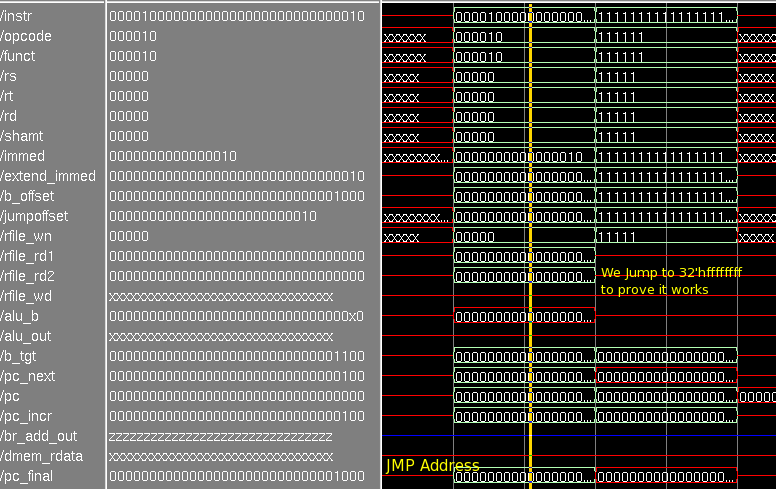
\includegraphics[scale=0.55]{img/jmp_wave.png}}

    \item
    Waveform diagram of the ADDI instruction.

    \centerline{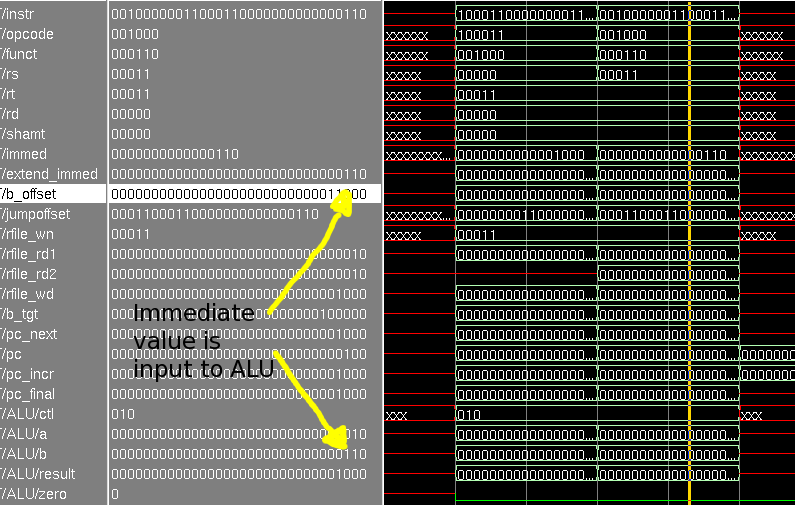
\includegraphics[scale=0.55]{img/addi_wave.png}}

    \item
    Waveform diagram of the BEQ instruction.

    \centerline{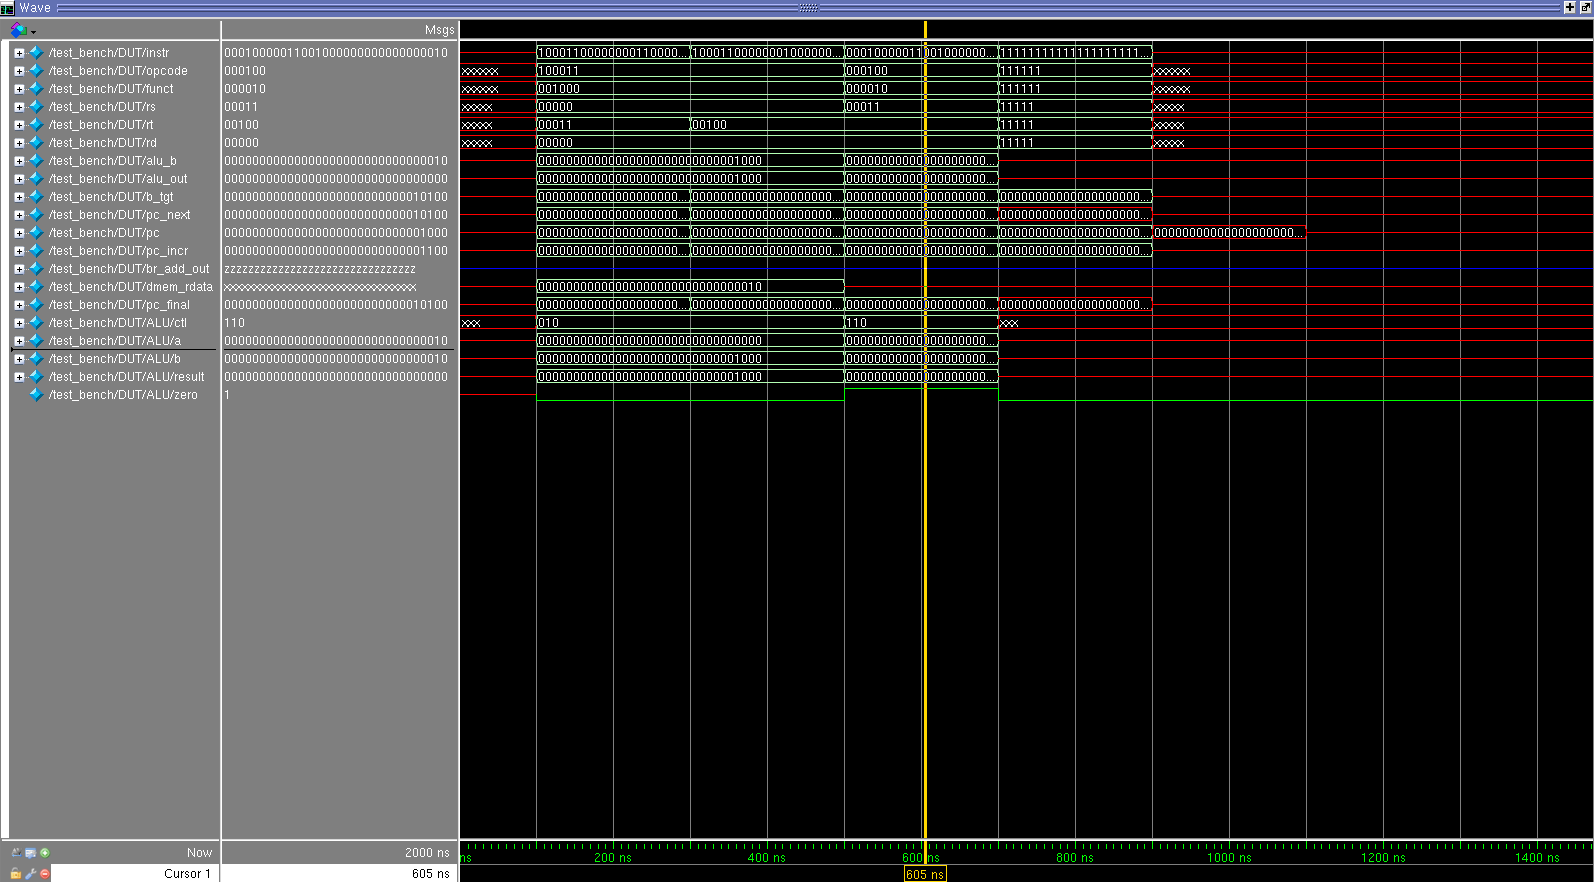
\includegraphics[scale=0.55]{img/beq_wave.png}}

    \item
    Waveform diagram of the BNE instruction.

    \centerline{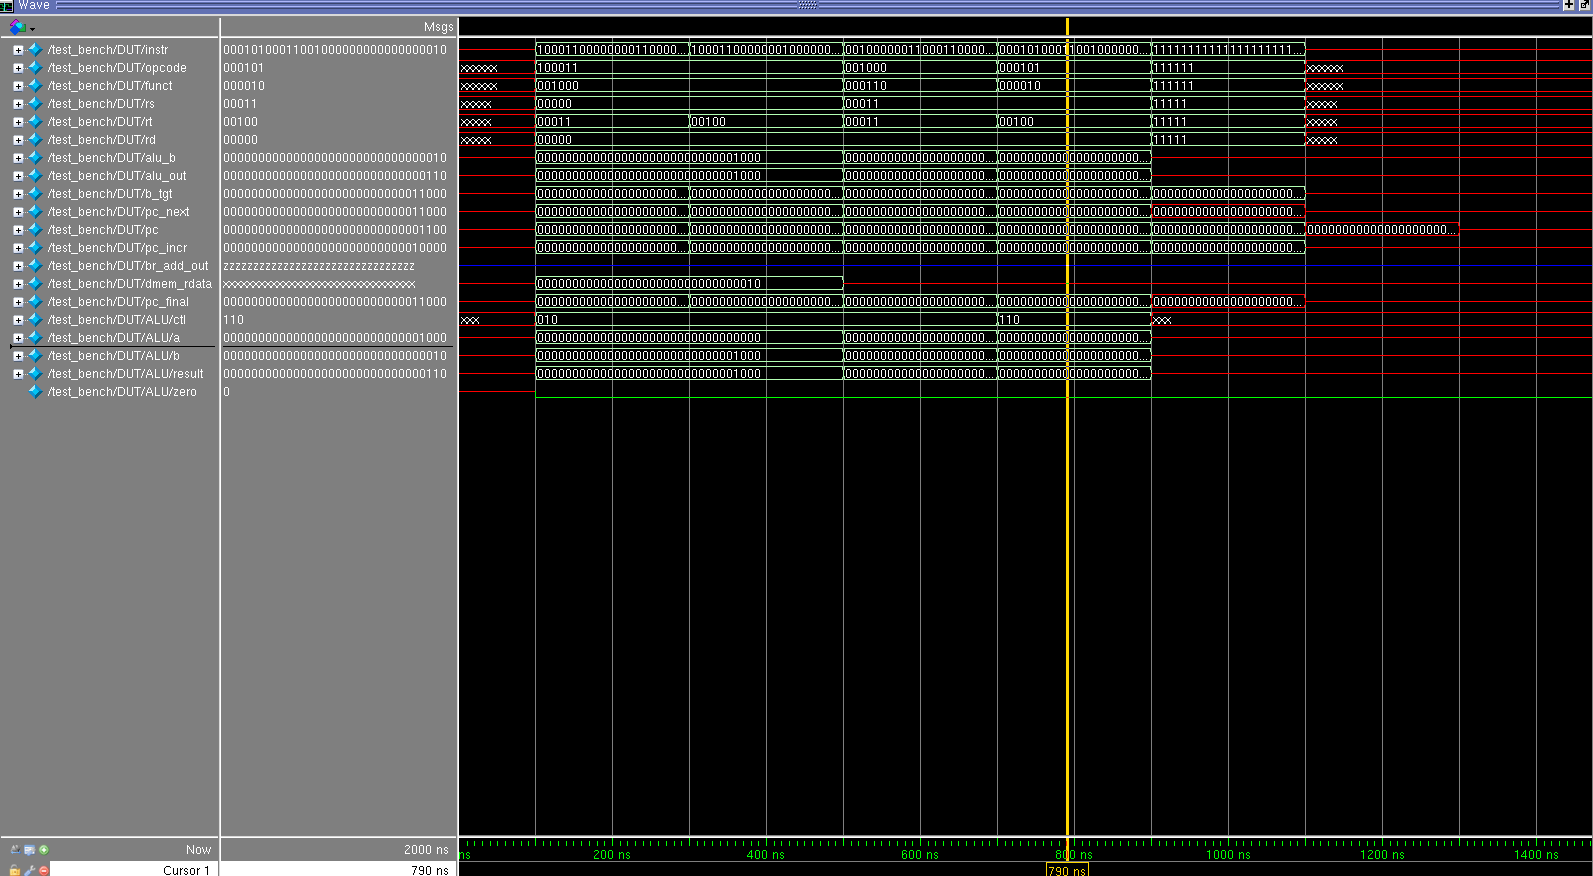
\includegraphics[scale=0.55]{img/bne_wave.png}}

\end{enumerate}

\section{Assembly Program}
\begin{verbatim}
        LW r3, 8(r0)
        LW r4, 8(r0)
        ADDI r4, r4, 6
        BEQ r3, r4, DONE ; LOOP
        ADDI r3, r3, 1
        JUMP LOOP
        ADDI r3, r3, 1 ; DONE
        BNE r3, r4, FINAL
        JUNK-INSTRUCTION:
        FINAL:
\end{verbatim}
    Waveform diagram of the test assembly program. The Signals have been truncated because they make the image too big. You can look at the previous figure to see the names of the signals.

    \centerline{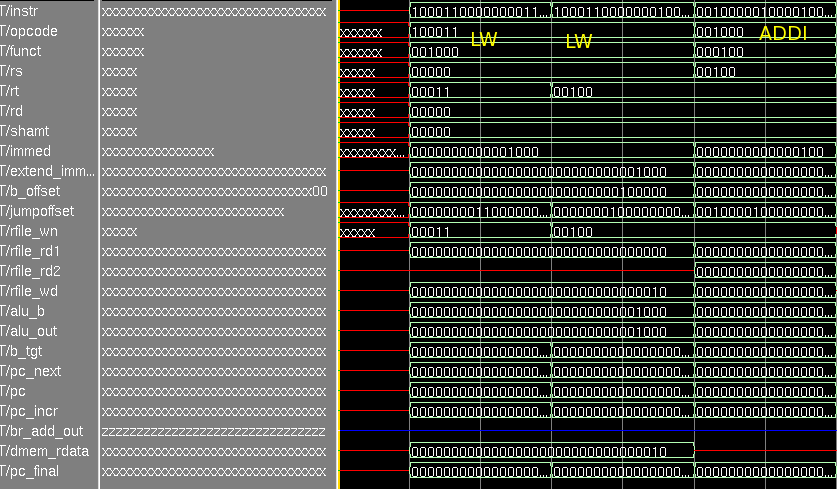
\includegraphics[scale=0.55]{img/test_program_wave_part1_1.png}}
    \centerline{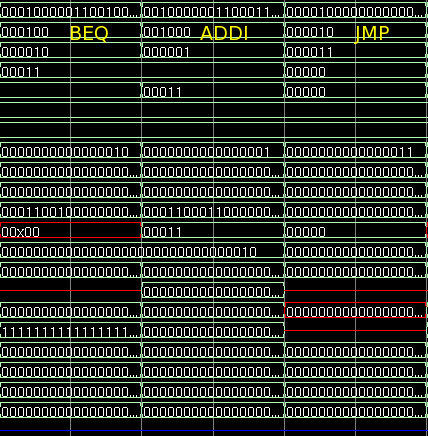
\includegraphics[scale=0.55]{img/test_program_wave_part1_2.png}}

    \centerline{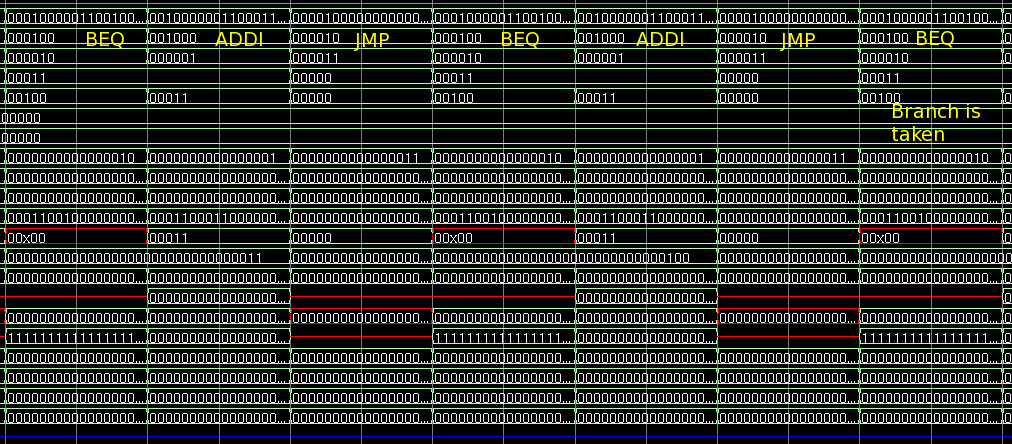
\includegraphics[scale=0.55]{img/test_program_wave_part2.png}}

    \centerline{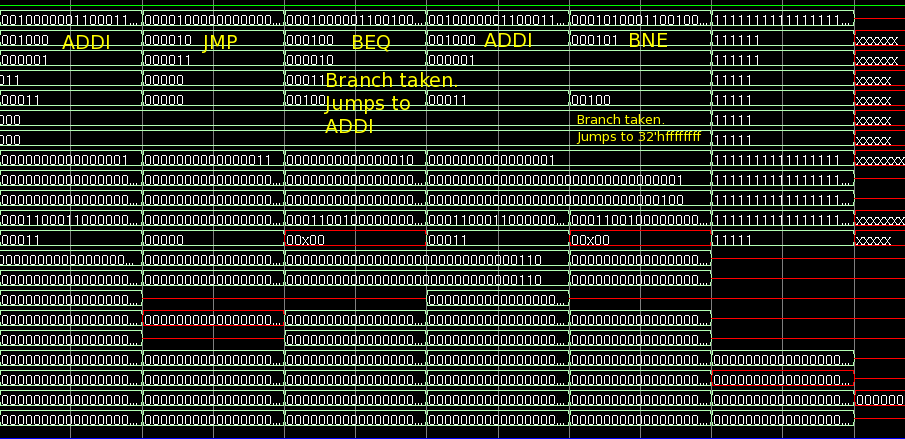
\includegraphics[scale=0.55]{img/test_program_wave_part3.png}}

\section{Modified ROM32 Code}
{\tiny
\begin{verbatim}
module rom32(address, data_out);
  input  [31:0] address;
  output [31:0] data_out;
  reg    [31:0] data_out;

  parameter BASE_ADDRESS = 25'd0; // address that applies to this memory

  wire [4:0] mem_offset;
  wire address_select;

  assign mem_offset = address[6:2];  // drop 2 LSBs to get word offset

  assign address_select = (address[31:7] == BASE_ADDRESS);  // address decoding

  always @(address_select or mem_offset)
  begin
    if ((address % 4) != 0) $display($time, " rom32 error: unaligned address %d", address);
    if (address_select == 1)
    begin
      case (mem_offset)

        /*
          // JUMP
          5'd0 : data_out = { 6'd2, 26'd2};                 // jmp
          5'd1 : data_out = { 6'd35, 5'd0, 5'd3, 16'd8 };   // lw $3, 8($0)   r3=2
          5'd2 : data_out = { 8'hff, 8'hff, 8'hff, 8'hff }; // lw $4, 20($0)  r4=5
        */

        /*
          // ADDI
          5'd0 : data_out = { 6'd35, 5'd0, 5'd3, 16'd8 };   // lw $3, 8($0)   r3=2
          5'd1 : data_out = { 6'd8, 5'd3, 5'd3, 16'd6 };    // addi $3, $3, 2
        */

        /*
          // BEQ
          5'd0 : data_out = { 6'd35, 5'd0, 5'd3, 16'd8 };   // lw $3, 8($0)   r3=2
          5'd1 : data_out = { 6'd35, 5'd0, 5'd4, 16'd8 };   // lw $4, 8($0)   r4=2
          5'd2 : data_out = { 6'd4,  5'd3, 5'd4, 16'd2 };   // beq r3, r4
          5'd3 : data_out = { 6'd35, 5'd0, 5'd3, 16'd8 };   //
          5'd4 : data_out = { 8'hee, 8'hee, 8'hee, 8'hee }; //
          5'd5 : data_out = { 8'hff, 8'hff, 8'hff, 8'hff }; // Target of beq
        */

        /*
          // BNE
          5'd0 : data_out = { 6'd35, 5'd0, 5'd3, 16'd8};    // lw $3, 8($0)   r3=2
          5'd1 : data_out = { 6'd35, 5'd0, 5'd4, 16'd8};    // lw $4, 20($0)   r4=2
          5'd2 : data_out = { 6'd8, 5'd3, 5'd3, 16'd6 };    // addi $3, $3, 6 r3=8
          5'd3 : data_out = { 6'd5,  5'd3, 5'd4, 16'd2};    // bne r3, r4
          5'd4 : data_out = { 6'd35, 5'd0, 5'd3, 16'd8 };   //
          5'd5 : data_out = { 8'hee, 8'hee, 8'hee, 8'hee }; //
          5'd6 : data_out = { 8'hff, 8'hff, 8'hff, 8'hff }; // Target of bne
        */

          // Test Program
          5'd0 : data_out = { 6'd35, 5'd0, 5'd3, 16'd8};    // lw $3, 8($0)  (r3=2)
          5'd1 : data_out = { 6'd35, 5'd0, 5'd4, 16'd8};    // lw $4, 8($0) (r4=2)

          5'd2 : data_out = { 6'd8, 5'd4, 5'd4, 16'd4 };    // addi $4, $4, 6 (r4=6)
          5'd3 : data_out = { 6'd4, 5'd3, 5'd4, 16'd2 };    // beq $3, $4, DONE ; LOOP
          5'd4 : data_out = { 6'd8, 5'd3, 5'd3, 16'd1 };    // addi $3, $3, 1
          5'd5 : data_out = { 6'd2, 26'd3 };                // JUMP LOOP
          5'd6 : data_out = { 6'd8, 5'd3, 5'd3, 16'd1 };    // addi $3, $3, 1 ; DONE
          5'd7 : data_out = { 6'd5,  5'd3, 5'd4, 16'd1 };   // bne $3, $4, FINAL
          5'd8 : data_out = { 8'hee, 8'hee, 8'hee, 8'hee }; //
          5'd9 : data_out = { 8'hff, 8'hff, 8'hff, 8'hff }; // FINAL:

          // add more cases here as desired
          default data_out = 32'hxxxx;
      endcase
      $display($time, " reading data: rom32[%h] => %h", address, data_out);
    end
  end
endmodule
\end{verbatim}
}

\section{Modified Datapath Code}
{\tiny
\begin{verbatim}
module mips_single(clk, reset);
    input clk, reset;

    // instruction bus
    wire [31:0] instr;

    // break out important fields from instruction
    wire [5:0] opcode, funct;
    wire [4:0] rs, rt, rd, shamt;
    wire [15:0] immed;
    wire [31:0] extend_immed, b_offset;
    wire [25:0] jumpoffset;

    assign opcode = instr[31:26];
    assign rs = instr[25:21];
    assign rt = instr[20:16];
    assign rd = instr[15:11];
    assign shamt = instr[10:6];
    assign funct = instr[5:0];
    assign immed = instr[15:0];
    assign jumpoffset = instr[25:0];

    // sign-extender
    assign extend_immed = { {16{immed[15]}}, immed };

    // branch offset shifter
    assign b_offset = extend_immed << 2;

    // datapath signals
    wire [4:0] rfile_wn;
    wire [31:0] rfile_rd1, rfile_rd2, rfile_wd, alu_b, alu_out, b_tgt, pc_next,
                pc, pc_incr, br_add_out, dmem_rdata, pc_final;

    // control signals

    wire RegWrite, Branch, PCSrc, RegDst, MemtoReg, MemRead, MemWrite, ALUSrc, Zero, Jump, sub_zero;
    wire [1:0] ALUOp;
    wire [2:0] Operation;

    // module instantiations

    reg32		PC(clk, reset, pc_final, pc);

    add32 		PCADD(pc, 32'd4, pc_incr);

    add32 		BRADD(pc_incr, b_offset, b_tgt);

    reg_file	RFILE(clk, RegWrite, rs, rt, rfile_wn, rfile_rd1, rfile_rd2, rfile_wd);

    alu 		ALU(Operation, rfile_rd1, alu_b, alu_out, Zero);

    rom32 		IMEM(pc, instr);

    mem32 		DMEM(clk, MemRead, MemWrite, alu_out, rfile_rd2, dmem_rdata);
                //     output in0     in1
    and  		BR_AND(PCSrc, Branch, sub_zero);

    mux2 #(5) 	RFMUX(RegDst, rt, rd, rfile_wn);

    mux2 #(32)	PCMUX(PCSrc, pc_incr, b_tgt, pc_next);

    mux2 #(32) 	ALUMUX(ALUSrc, rfile_rd2, extend_immed, alu_b);

    mux2 #(32)	WRMUX(MemtoReg, alu_out, dmem_rdata, rfile_wd);

    // Extend MIPS datapath to handle jump instruction by adding a mux
    // to choose between branch target and jump address.
    mux2 #(32)  JUMPMUX(Jump, pc_next, {pc_incr[31:28], jumpoffset, 2'b00}, pc_final);

    // BEQ 00010(0) Zero
    // BNE 00010(1) NOT Zero
    mux2 #(1)   BRMUX(opcode[0], Zero, ~Zero, sub_zero);

    control_single CTL(.opcode(opcode), .RegDst(RegDst), .ALUSrc(ALUSrc), .MemtoReg(MemtoReg),
                       .RegWrite(RegWrite), .MemRead(MemRead), .MemWrite(MemWrite), .Branch(Branch),
                       .ALUOp(ALUOp), .Jump(Jump));

    alu_ctl 	ALUCTL(ALUOp, funct, Operation);
endmodule
\end{verbatim}
}

\section{Control Signals Code}
{\tiny
\begin{verbatim}
module control_single(opcode, RegDst, ALUSrc, MemtoReg, RegWrite, MemRead, MemWrite, Branch, ALUOp, Jump);
    input [5:0] opcode;
    output RegDst, ALUSrc, MemtoReg, RegWrite, MemRead, MemWrite, Branch, Jump;
    output [1:0] ALUOp;
    reg    RegDst, ALUSrc, MemtoReg, RegWrite, MemRead, MemWrite, Branch, Jump;
    reg    [1:0] ALUOp;

    parameter R_FORMAT = 6'd0;
    parameter LW = 6'd35;
    parameter SW = 6'd43;
    parameter BEQ = 6'd4;

    parameter JMP = 6'd2;
    parameter ADDI = 6'd8;
    parameter BNE = 6'd5;

    always @(opcode)
    begin
        case (opcode)
          R_FORMAT :
          begin
              RegDst=1'b1; ALUSrc=1'b0; MemtoReg=1'b0; RegWrite=1'b1; MemRead=1'b0;
              MemWrite=1'b0; Branch=1'b0; ALUOp = 2'b10; Jump=0;
          end
          LW :
          begin
              RegDst=1'b0; ALUSrc=1'b1; MemtoReg=1'b1; RegWrite=1'b1; MemRead=1'b1; MemWrite=1'b0; Branch=1'b0; ALUOp = 2'b00; Jump=0; end
          SW :
          begin
              RegDst=1'bx; ALUSrc=1'b1; MemtoReg=1'bx; RegWrite=1'b0; MemRead=1'b0;
              MemWrite=1'b1; Branch=1'b0; ALUOp = 2'b00; Jump=0;
          end
          BEQ :
          begin
              // RegDst: x, not writing to register
              // ALUSrc: 1, extend_immed
              // Memtoreg: x, not writing to register
              // RegWrite: 0, not writing to register
              // MemRead: 0, not reading from memory
              // MemWrite: 0, not writing to memory
              // Branch: 1,
              // ALUOp: 01, subtract to compare
              RegDst=1'bx; ALUSrc=1'b0; MemtoReg=1'bx; RegWrite=1'b0; MemRead=1'b0;
              MemWrite=1'b0; Branch=1'b1; ALUOp=2'b01; Jump=0;
          end
          JMP :
          begin
              // RegDst: x, not writing to register
              // ALUSrc: 1, extend_immed
              // Memtoreg: x, not writing to register
              // RegWrite: 0, not writing to register
              // MemRead: 0, not reading from memory
              // Branch: 1, set new PC
              // ALUOp: xx
              // Jump: 1, to jump address, not branch target
              $display("BEGIN JUMP PREP");
              RegDst=1'bx; ALUSrc=1'bx; MemtoReg=1'bx; RegWrite=1'b0; MemRead=1'b0;
              MemWrite=1'b0; Branch=1'b1; ALUOp = 2'bxx; Jump=1'b1;
          end
          ADDI :
          begin
              // RegDst: 0, write to rt
              // ALUSrc: 1, read from second register port
              // Memtoreg: 0, ALU result to register
              // RegWrite: 1, writing to register
              // MemRead: 0, not reading from memory
              // Branch: 0, not branching
              // ALUOp: 00, add two registers
              RegDst=1'b0; ALUSrc=1'b1; MemtoReg=1'b0; RegWrite=1'b1; MemRead=1'b0;
              MemWrite=1'b0; Branch=1'b0; ALUOp=2'b00; Jump=0;
          end
          BNE :
          begin
              // RegDst: x, not writing to register
              // ALUSrc: 1, extend_immed
              // Memtoreg: x, not writing to register
              // RegWrite: 0, not writing to register
              // MemRead: 0, not reading from memory
              // MemWrite: 0, not writing to memory
              // Branch: 1,
              // ALUOp: 01, subtract to compare
              RegDst=1'bx; ALUSrc=1'b0; MemtoReg=1'bx; RegWrite=1'b0; MemRead=1'b0;
              MemWrite=1'b0; Branch=1'b1; ALUOp=2'b01; Jump=0;
          end
          default
          begin
              $display("control_single unimplemented opcode %d", opcode);
              RegDst=1'bx; ALUSrc=1'bx; MemtoReg=1'bx; RegWrite=1'bx; MemRead=1'bx;
              MemWrite=1'bx; Branch=1'bx; ALUOp = 3'bxxx; Jump=0;
          end

        endcase
    end
endmodule
\end{verbatim}
}

\end{document}
